%% GenSIE 2026 Working Notes -- SEsml system description
%% CEURART format (one column)
\documentclass{ceurart}

\usepackage{listings}
\usepackage{booktabs}
\usepackage{xspace}
\usepackage{url}

\lstset{
  breaklines=true,
  basicstyle=\ttfamily\small,
  columns=fullflexible,
}

%% Fix overfulls
\sloppy

\begin{document}

%% Rights management
\copyrightyear{2026}
\copyrightclause{Copyright for this paper by its authors.
  Use permitted under Creative Commons License Attribution 4.0
  International (CC BY 4.0).}

%% Conference information
\conference{IberLEF 2026, September 2026, Le\'on, Spain}

%% Title
\title{SEsml: Schema-guided Extraction with Small Language Models}

%% Authors
\author[1]{Alejandro Beltr\'an}[%
  orcid=0009-0009-8073-1033,
  email=alejandro.beltran@rect.uh.cu,
]
\address[1]{Universidad de La Habana, Havana, Cuba}

%% Abstract
\begin{abstract}
This paper presents \textbf{SEsml} (Schema-guided Extraction with Small Language Models),
a particular solution submitted by a researcher at the Universidad de La Habana
to the GenSIE 2026 shared task at IberLEF 2026.
The task requires zero-shot extraction of nested JSON objects from Spanish texts using
SLMs under 14B parameters.
SEsml instantiates a central design principle --- \emph{decoupling semantic reasoning
from structural enforcement} --- as its defining architectural choice.
The system argues that constrained decoding, while guaranteeing syntactic validity,
imposes a measurable \emph{constraint tax} on small models that degrades semantic accuracy.
To mitigate this, the principal pipeline, \emph{extraction}, employs a two-phase
draft-then-decode architecture that makes the decoupling explicit: an unconstrained
DraftEngine produces a semi-structured \texttt{campo: valor} representation, followed
by a Constrained Decoder that maps the draft into schema-valid JSON under
\texttt{response\_format=json\_schema}.
Two lighter variants explore alternative trade-offs: \emph{hybrid\_cot} (single-call with
visible chain-of-thought) and \emph{adaptive} (task-adaptive prompt assembly via semantic
similarity).
All pipelines share a SchemaOptimizer that resolves \$ref references, enforces structural
constraints, and normalises schemas for constrained decoding engines.
The paper documents the prompt evolution from a verbose v1 ({\textasciitilde}3,180 chars)
to a compact v3b ({\textasciitilde}1,163 chars), finding that shorter, rule-based prompts
consistently outperform longer instructions for SLMs.
On the GenSIE 2026 development set (149 tasks),
all three SEsml pipelines outperform the unconstrained baseline on both
Gemma 4 E4B and Qwen3-14B, closing 13.4--43.6\% of the gap to a perfect system.
The extraction pipeline is most effective on the smaller Gemma model (gap-closed 0.1761),
while the adaptive pipeline leads on Qwen3-14B (gap-closed 0.4363).
The SEsml team placed 5th of 11 teams on the official leaderboard (mean GapClosed = 0.0481).
\end{abstract}

%% Keywords
\begin{keywords}
structured extraction \sep
small language models \sep
constrained decoding \sep
schema-guided generation \sep
Spanish NLP \sep
draft-then-decode
\end{keywords}

\maketitle

%% =======================================================================
\section{Introduction}
%% =======================================================================

The extraction of structured information from unstructured text is a fundamental task
in natural language processing, underpinning applications from knowledge base
construction to document understanding.
While large language models (LLMs) have demonstrated remarkable capabilities in
open-ended text generation, reliably extracting structured data --- particularly in
formats such as JSON --- remains challenging, especially when using small language
models (SLMs) that are practical for on-device or resource-constrained deployments.

The GenSIE (General-purpose Schema-guided Information Extraction) shared task, hosted
at IberLEF 2026 \cite{iberlef2026overview}, addresses this challenge head-on
\cite{gensie2026overview}.
Participants must build systems that take a Spanish text fragment and an arbitrary
JSON Schema, and produce a valid JSON object whose values are faithfully grounded
in the input.
The task is zero-shot: test schemas may be entirely unseen during development.
All systems must use SLMs with fewer than 14 billion parameters, reflecting the
realistic constraint that such models must be deployable on consumer hardware.

This paper presents \textbf{SEsml} (Schema-guided Extraction with Small Language
Models), a particular solution submitted by the ExtractUH team of the Universidad
de La Habana to the GenSIE 2026 shared task.
SEsml comprises three complementary pipelines --- \emph{extraction}, \emph{hybrid\_cot},
and \emph{adaptive} --- all of which instantiate the same defining architectural choice:
\emph{decoupling semantic reasoning from structural enforcement}.

The motivation for this principle arises from a well-documented limitation of constrained
decoding.
While techniques such as token masking and grammar-guided generation guarantee
syntactically valid output, they impose a measurable \emph{constraint tax}
\cite{Castillo2025} on small models.
When forced to simultaneously reason about content and maintain rigid JSON syntax,
SLMs suffer from \emph{capacity contention}: their limited representational capacity
is split between semantic accuracy and syntactic compliance, degrading both.
Recent work on \emph{Draft-Conditioned Constrained Decoding} \cite{Reddy2026} and
\emph{In-Writing} \cite{Nguyen2026} demonstrates that generating an unconstrained
intermediate representation before applying structural constraints can substantially
mitigate this degradation.

The principal pipeline, \emph{extraction}, operationalises this insight through a
two-phase architecture that makes the decoupling explicit: an unconstrained
DraftEngine produces a semi-structured \texttt{campo: valor} representation without
JSON syntax, followed by a Constrained Decoder that maps the draft into schema-valid
JSON using \texttt{response\_format=json\_schema}.
Two lighter variants --- \emph{hybrid\_cot} (single-call with visible chain-of-thought)
and \emph{adaptive} (task-adaptive prompt assembly via semantic similarity) --- explore
alternative trade-offs between decoupling, latency, and schema complexity.

The pipelines are evaluated on the GenSIE development set (149 tasks) and the official
test set (145 tasks) across two SLM families (Gemma 4 E4B, Qwen3-14B).
On the development set, all three SEsml pipelines outperform the unconstrained baseline
on both models.
The extraction pipeline closes 17.6\% of the gap to perfect on Gemma 4 E4B, while the
adaptive pipeline achieves the best overall score on Qwen3-14B (gap-closed 0.4363).
On the official leaderboard, the SEsml team placed 5th of 11 systems with a mean
GapClosed of 0.0481.

The paper is organised as follows.
Section~\ref{sec:background} provides background on constrained decoding limitations
and the draft-then-decode solution.
Section~\ref{sec:architecture} presents the overall system architecture.
Section~\ref{sec:schema-optimization} details the schema optimisation approach.
Section~\ref{sec:extraction} describes the principal extraction pipeline.
Section~\ref{sec:alternatives} covers the alternative pipelines.
Section~\ref{sec:prompts} discusses prompt engineering and the evolution of the
prompt design.
Section~\ref{sec:results} presents experimental results,
Section~\ref{sec:error-analysis} analyses error patterns, and
Section~\ref{sec:conclusions} concludes.

%% =======================================================================
\section{Background: The Challenge of Constrained Decoding for Small Language Models}
\label{sec:background}
%% =======================================================================

\subsection{Problem Setup}

The GenSIE shared task requires systems to perform zero-shot extraction of nested
JSON objects from general-domain Spanish texts, using language models with fewer
than 14 billion parameters.
For each instance, the system receives a text fragment, a natural-language instruction,
and an arbitrary target schema defined as a JSON Schema (OpenAPI 3.0 subset).
The output must be a valid JSON object that strictly conforms to the schema while
containing only information faithfully extracted from the input text --- returning
\texttt{null} for any field whose value is not present.

This setting imposes three simultaneous demands on the model:
(a)~understand and reason about the Spanish input text, which may require resolving
coreferences, handling rich morphology, and performing multi-hop inference across
paragraphs;
(b)~interpret the target schema, which may include nested objects, enumerated types
with strict case-sensitive matching, inter-field constraints, and hallucination traps
where fields request plausible but absent information; and
(c)~produce syntactically perfect JSON, where a single misplaced comma, unescaped
quote, or type mismatch renders the output unusable.

For small language models (SLMs) with limited representational capacity, these demands
compete for the same finite cognitive budget --- what the authors term
\emph{capacity contention}.

\subsection{Why Constrained Decoding: A Task-Driven Necessity}

The GenSIE task specification imposes a hard requirement: every output must be a
syntactically valid JSON object conforming to the target schema.
An output whose JSON cannot be parsed --- due to a misplaced comma or unescaped quote
--- yields a structural failure that the scoring metric cannot evaluate, effectively
scoring zero for that instance.
While the Flattened Schema Scoring does credit partially valid structures through its
key-wise evaluation, a single unparseable output loses an entire instance's
contribution to the final F1.
For a shared task where every percentage point matters, unreliable syntax is a
liability no competitive system can afford.

This is not merely a stylistic preference.
Castillo~\cite{Castillo2025} reports that across diverse extraction tasks,
unconstrained SLMs (no \texttt{response\_format} enforcement) produce syntactically
valid JSON on only 60--70\% of instances.
The remaining 30--40\% of outputs --- containing trailing commas, unquoted keys,
truncated objects, or extraneous text --- are structurally useless regardless of
their semantic content.
For a system competing on F1, syntactic failure is catastrophic: it nullifies any
semantic accuracy the model may have achieved.

Constrained decoding (CD) addresses this failure mode directly.
At each generation step, CD intervenes at the token level, masking any continuation
that would violate the target grammar or schema and renormalising over the remaining
valid set \cite{Willard2023, Geng2023}.
Tools such as Outlines, XGrammar \cite{Dong2024}, and OpenAI's
\texttt{response\_format=json\_schema} compile JSON schemas into finite-state machines
that enforce structural correctness token by token.
The result is predictable and well-documented: schema validity rises from the
unconstrained baseline of 60--70\% to effectively 100\%, eliminating syntax errors,
missing fields, and extraneous commentary \cite{Castillo2025}.
Modern engines achieve this with minimal latency overhead --- XGrammar reports
near-zero added cost per token \cite{Dong2024}, and coalescence techniques can even
accelerate generation by up to 50\% over unconstrained decoding by skipping
deterministic scaffolding \cite{Geng2025, Kurt2024}.

These properties make CD one of the most viable options for the GenSIE task: no system
that accepts 30--40\% structural failure rates can be competitive in a shared task
where every percentage point of F1 matters.
SEsml therefore adopts constrained decoding as its structural backbone --- but with
full awareness that CD is not a free lunch.
The same mechanism that guarantees syntactic validity also imposes a measurable
\emph{constraint tax} on semantic accuracy, particularly for small models.
The following subsections analyse this tax and present the mitigation strategies that
are the paper's central contribution.

\subsection{The Constraint Tax}

However, CD is not a passive formatting filter.
Because it intervenes at every generation step, it alters the model's internal
probability distribution in ways that can degrade semantic accuracy.
This phenomenon, termed the \emph{constraint tax}, is particularly severe for
small models.

Reddy et al.~\cite{Reddy2026} formalise the mechanism through a KL-divergence lens:
at each step, CD projects the model's original distribution onto the set of valid
continuations via reverse-KL minimisation.
When the model assigns low probability to valid tokens --- which is typical when
generating rigid syntax tokens such as braces, commas, or field names --- this
projection constitutes a large perturbation.
Repeating this perturbation over hundreds of steps induces a cumulative
\emph{projection tax} that systematically biases decoding toward locally valid but
semantically incorrect trajectories.

The empirical magnitude of the constraint tax is striking.
Castillo~\cite{Castillo2025} conducted a controlled 15,000-generation study comparing
unconstrained prompting with hard schema-constrained decoding on SLMs.
Hard CD raised schema validity from 61.5\% to 100.0\%, but simultaneously lowered
answer accuracy from 19.7\% to 11.0\%.
The proportion of outputs that were structurally valid but semantically wrong rose
from 49.5\% to 88.9\% --- the model produced \emph{more} wrong answers precisely
because it was forced into valid JSON.
Schall and De Melo~\cite{Schall2025} independently confirmed this effect across
diverse model architectures and task types, showing that constraint-induced
performance degradation is inversely correlated with model scale: smaller models
suffer disproportionately larger accuracy drops under identical constraints.

\subsection{Capacity Contention and Structure Snowballing}

The constraint tax manifests through two interrelated failure modes directly observed
during system development.

\textbf{Capacity contention} occurs when an SLM attempts to reason about semantic
content while simultaneously maintaining rigid JSON syntax.
The model's limited representational capacity forces a trade-off: attention devoted
to tracking open braces, comma placement, and quote escaping is attention withdrawn
from entity recognition, relationship extraction, and value verification.
This is not merely a prompting issue --- it is a fundamental consequence of
autoregressive generation under conflicting objectives.

\textbf{Structure snowballing}, identified by Zhou et al.~\cite{Zhou2025}, represents
an even more insidious failure.
Under Outlines-based constrained decoding, the cognitive load of formatting compliance
can push the model into \emph{formatting traps} --- repetitive, self-reinforcing
cycles of syntactic correction that consume generation capacity without resolving the
underlying semantic errors.
The model achieves perfect superficial syntactic alignment while entirely missing deep
semantic errors.
Zhou et al.~term this the \emph{alignment tax} of constrained decoding: a tension
between structural granularity and internal model capacity.

Nguyen et al.~\cite{Nguyen2026} demonstrated that this fragility extends beyond
grammar-level constraints to simple lexical ones.
Instruction-tuned models suffered 14--48\% comprehensiveness loss when asked to avoid
a single common word or punctuation character.
Through mechanistic analysis, they identified this as a \emph{planning failure}: the
instruction-tuned model's response template was disrupted by the constraint, causing
it to abandon its normal reasoning process.
Notably, base (non-instruction-tuned) models showed no systematic collapse,
confirming that instruction tuning itself creates the coupling between task competence
and narrow surface-form templates.

\subsection{Draft-then-Decode: Decoupling Reasoning from Formatting}

A growing body of work demonstrates that these failure modes can be mitigated by
\emph{decoupling} the reasoning phase from the formatting phase.
The key insight is that if a model can express its understanding in a natural,
unconstrained form before being required to produce structured output, the syntactic
constraints no longer compete for the same cognitive budget.

Reddy et al.~\cite{Reddy2026} propose \emph{Draft-Conditioned Constrained Decoding}
(DCCD), a training-free two-stage procedure.
In the first stage, a model generates an unconstrained draft --- free text, reasoning
steps, or semi-structured notes --- capturing the semantic plan.
In the second stage, constrained decoding is applied \emph{conditioned on this draft},
so that the model primarily performs structured realisation rather than open-ended
reasoning.
The draft shifts probability mass toward schema-consistent continuations,
substantially reducing the projection tax.
Across GSM8K, MATH500, and FOLIO benchmarks with models ranging from 1B to 14B
parameters, DCCD improved structured accuracy by up to +24 percentage points over
standard CD (e.g., 15.2\% to 39.0\% on GSM8K with a 1B model).
Critically, the second stage could often be performed by a smaller model, enabling
parameter-efficient composition.

Nguyen et al.~\cite{Nguyen2026} propose \emph{In-Writing}, a complementary approach
that allows models to reason freely in natural language until a trigger token (such as
\texttt{\{} or \texttt{<eos>}) switches the decoder to structured generation.
This hybrid decoding preserves the expressive power of natural language reasoning while
ensuring structured output reliability, achieving up to 27\% accuracy gains on
reasoning tasks with minimal token overhead (10--20 extra tokens).

Cooper~\cite{Cooper2024} observes a simpler instantiation of the same principle in
schema design: placing reasoning or explanation fields before answer fields in a
JSON schema preserves chain-of-thought quality, because the model generates fields
left-to-right and can reason before committing to a final answer.
Commercial providers have adopted similar recommendations, with field ordering
emerging as a best practice for structured output APIs \cite{Tam2024}.

\subsection{Proposed design}

Drawing on these findings, the three pipelines presented in this paper embody a
\emph{think-first, format-later} design philosophy.
The principal extraction pipeline (Section~\ref{sec:extraction}) takes the most
explicit form of decoupling with two dedicated stages: an unconstrained DraftEngine
that produces a semi-structured \texttt{campo: valor} representation without JSON
syntax, followed by a Constrained Decoder that maps this draft into schema-valid
JSON under \texttt{response\_format=json\_schema}.
The hybrid\_cot and adaptive pipelines (Section~\ref{sec:alternatives}) achieve
similar decoupling within a single LLM call by placing visible chain-of-thought
reasoning (\texttt{<Thinking>...</Thinking>}) before the structured output,
allowing the model to reason without the overhead of JSON syntax before committing
to the final format.

This architectural choice is motivated by the specific constraints of the GenSIE task:
Spanish text extraction with SLMs under 14B parameters, where the constraint tax is
most pronounced and the benefits of decoupling are correspondingly largest.
The following section presents the resulting system architecture.

%% =======================================================================
\section{System Architecture}
\label{sec:architecture}
%% =======================================================================

All three SEsml pipelines share a common philosophy --- \emph{think first, format
later} --- rooted in the analysis of Section~\ref{sec:background}.
They differ in how explicitly they separate reasoning from formatting, ranging from
two explicit LLM calls (extraction) to implicit separation within a single call
(hybrid\_cot, adaptive).
They also share a preprocessing stage --- SchemaOptimizer --- that transforms arbitrary
JSON Schema inputs into a canonical form suitable for both prompting and constrained
decoding.

\subsection{Architectural Overview}

Figure~\ref{fig:architecture} illustrates the high-level architecture common to all
pipelines.

\begin{figure}
  \centering
  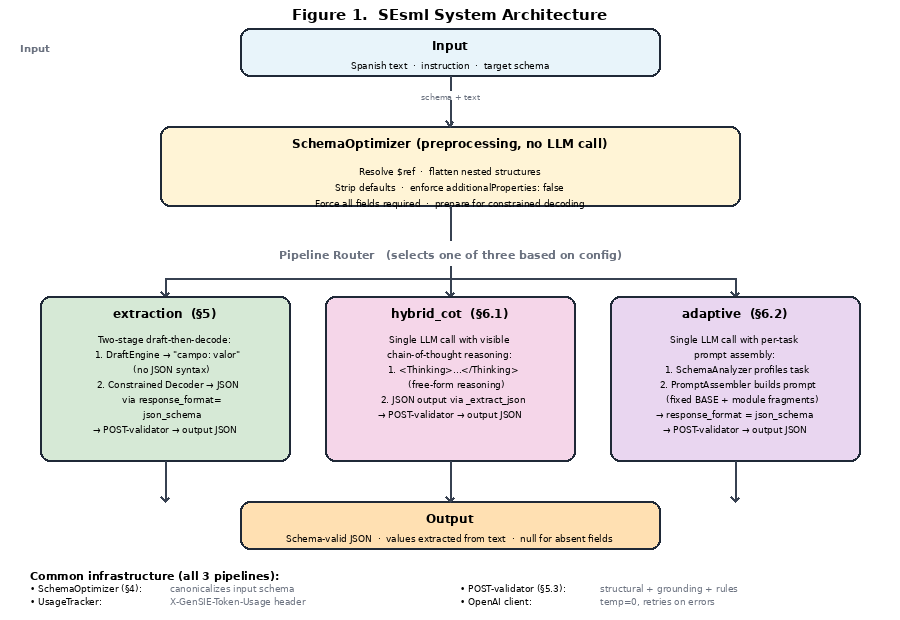
\includegraphics[width=\linewidth]{figure-1-architecture.png}
  \caption{System architecture.
    All input schemas pass through the SchemaOptimizer, then are routed to the
    selected pipeline.
    The extraction pipeline uses two LLM calls; hybrid\_cot and adaptive use one.
    The legend at the bottom lists the components that are shared by all three
    pipelines.}
  \label{fig:architecture}
\end{figure}

\subsection{Common Infrastructure}

All pipelines share the following infrastructure:

\textbf{Model-agnostic client.}
Every pipeline uses an OpenAI-compatible HTTP client that respects the \texttt{model}
parameter passed by the evaluator at runtime.
This is a hard requirement of the GenSIE evaluation protocol, which tests each
pipeline against multiple models including held-out ones.
The client implements retry logic with exponential backoff and a configurable timeout.

\textbf{Inference configuration.}
All LLM calls use \texttt{temperature=0} (greedy decoding) and disable streaming
(\texttt{stream: false}), as required by the evaluation specification.
The maximum output token limit is set to 4096 per call, which is sufficient for the
schema sizes in GenSIE without excessive token consumption.

\textbf{Usage tracking.}
Each pipeline tracks token usage via \texttt{gensie.usage.UsageTracker}, which reports
cumulative input, output, and total tokens per instance through the
\texttt{X-GenSIE-Token-Usage} response header.
This is required for the efficiency leaderboard and for transparency against the
server-side usage log.

\textbf{POST-validation.}
All pipeline outputs pass through a three-layer verifier (Section~\ref{sec:extraction})
that checks structural validity, value grounding, and inter-field business rules.
This is independent of the constrained decoding mechanism and serves as a final
quality gate.

\subsection{Pipeline Comparison}

\begin{table}
  \caption{Pipeline comparison across key dimensions.}
  \label{tab:pipeline-comparison}
  \centering
  \small
  \begin{tabular}{lccc}
    \toprule
    Dimension & Extraction (\S5) & HybridCoT (\S6.1) & Adaptive (\S6.2) \\
    \midrule
    LLM calls       & 2                         & 1                  & 1 \\
    Decoupling      & Explicit (two stages)     & Implicit (CoT)     & Implicit (prompt) \\
    Constraint      & \texttt{json\_schema}     & \texttt{\_extract} & \texttt{json\_schema} \\
    Prompt strategy & Fixed, minimal            & Fixed, minimal     & Assembled per task \\
    Best for        & Complex schemas           & Simpler schemas    & Diverse domains \\
    Schema preproc  & SchemaOptimizer           & SchemaOptimizer    & SchemaOptimizer + SchemaAnalyzer \\
    \bottomrule
  \end{tabular}
\end{table}

The following sections describe each component in detail, starting with the shared
SchemaOptimizer (Section~\ref{sec:schema-optimization}), then the principal extraction
pipeline (Section~\ref{sec:extraction}), and finally the alternative pipelines
(Section~\ref{sec:alternatives}).

%% =======================================================================
\section{Schema Optimization}
\label{sec:schema-optimization}
%% =======================================================================

The GenSIE task provides target schemas as JSON Schema objects conforming to the
OpenAPI 3.0 subset.
These schemas can contain features that are problematic for both prompt-based
extraction and constrained decoding engines: \$ref references requiring resolution,
optional fields that increase the state space of finite-state machines, numeric
constraints that complicate grammar compilation, and metadata fields such as
\texttt{title}, \texttt{default}, and \texttt{format} that can confuse small models
during prompting.

The \textbf{SchemaOptimizer} is a local (no LLM call) preprocessing component that
transforms the raw schema into a canonical form optimised for both downstream stages.
It operates as a pure function: given a raw schema dictionary, it returns a
\texttt{CleanSchema} object containing the cleaned schema, a list of
\texttt{FieldMetadata} entries for prompt construction, and error information.

\subsection{Resolution and Flattening}

\texttt{\$ref} resolution.
The optimizer recursively resolves \$ref pointers by following definitions within the
schema's \$defs or definitions sections.
This is essential for constrained decoding engines that operate on a single flat
schema --- unresolved references cause compilation failures in tools such as
Outlines' FSM builder.
The resolution is performed inline, producing self-contained nested schema definitions.

\textbf{Structure flattening.}
While schemas are not fully flattened (nested objects are preserved since they define
the output structure), the optimizer ensures that every nested level is independently
valid.
It also strips \$defs sections after resolution since they are no longer needed,
reducing token count.

\subsection{Cleaning Operations}

The optimizer applies the following cleaning transformations:

The optimizer annotates every object-level schema with \texttt{"additionalProperties": false},
forcing the constrained decoding engine to reject any field not explicitly listed in
\texttt{properties}.
This prevents the model from hallucinating extra fields --- a common failure mode in
schema-guided generation.

\textbf{Force all properties required.}
The optimizer sets every property as \texttt{required} by adding all property names to
the \texttt{required} array if not already present.
This serves two purposes: it reduces the FSM state space (optional fields would double
the branching factor at each object level), and it forces the model to explicitly
produce \texttt{null} for missing information rather than omitting the key entirely
--- which is required by the GenSIE scoring metric.

\textbf{Strip unsafe keys.}
Keys that interfere with prompting or constrained decoding are removed:
\texttt{default} (can bias the model toward fabricated values), \texttt{title}
(redundant with the field name), \texttt{format} (date-format hints that conflict
with Spanish locale conventions), and numeric constraints such as \texttt{minimum},
\texttt{maximum}, \texttt{minLength}, \texttt{maxLength} (these add grammar complexity
without corresponding benefit for extraction tasks).

\textbf{Enum normalisation.}
Enum values are preserved exactly as specified, including case sensitivity.
No normalisation is applied, since the GenSIE scoring requires exact match for enum
fields.
The optimizer extracts enum values into the field metadata for explicit inclusion in
prompts.

\subsection{Field Metadata Extraction}

Alongside the cleaned schema, the optimizer produces a list of \texttt{FieldMetadata}
objects --- one per leaf field in the flattened schema tree --- containing:

\begin{itemize}
\item \textbf{Field path} in dot notation (e.g., \texttt{event.city})
\item \textbf{Type} (string, integer, number, boolean, array, object)
\item \textbf{Enum values} (if present)
\item \textbf{Description} (the schema \texttt{description} field, which often contains
  critical extraction guidance)
\item \textbf{Required status} (always true after optimisation)
\item \textbf{Inference flag}: whether the schema \texttt{description} contains
  keywords such as \texttt{reasoned}, \texttt{inferred}, \texttt{based on}, or
  \texttt{classify}, indicating that the field value must be inferred rather than
  extracted verbatim
\end{itemize}

This metadata list is used by all three pipelines to construct field-level instructions
in prompts, ensuring that each field receives targeted guidance appropriate to its type
and semantics.

\subsection{Importance for Constrained Decoding}

Schema optimisation is particularly critical for the extraction pipeline's second stage
(Constrained Decoder) and the adaptive pipeline, both of which use
\texttt{response\_format=json\_schema}.
The optimizer's transformations directly address known limitations of FSM-based
constrained decoding engines:

\begin{itemize}
\item Resolved \$ref prevents compilation crashes.
\item \texttt{additionalProperties: false} prevents field hallucinations.
\item Forced \texttt{required} reduces branching and ensures \texttt{null} is explicit.
\item Cleaned metadata keeps prompts concise --- the active v3b prompt fits in
  {\textasciitilde}387 tokens, well within the budget for small models.
\end{itemize}

Without this preprocessing step, many raw GenSIE schemas --- particularly those with
cross-references --- would cause structured output calls to fail entirely.

%% =======================================================================
\section{Principal Pipeline: Draft-then-Decode}
\label{sec:extraction}
%% =======================================================================

The \emph{extraction} pipeline is the principal contribution.
It implements the draft-then-decode paradigm through two distinct LLM calls --- a
DraftEngine that produces a semi-structured intermediate representation, followed by
a Constrained Decoder that maps this draft into schema-valid JSON --- plus a
POST-validation layer.

\subsection{Phase 1: DraftEngine}

The DraftEngine is a single LLM call without any \texttt{response\_format} constraint
--- the model generates free-form text.
Its prompt consists of:

\begin{enumerate}
\item A brief system instruction setting the extraction task.
\item The input text and instruction.
\item The cleaned schema (from SchemaOptimizer).
\item A request to produce output in \texttt{<Thinking>...</Thinking><Draft>...</Draft>}
  format.
\end{enumerate}

The model is asked to first think about the task within \texttt{<Thinking>} tags, then
produce a semi-structured draft in \texttt{campo: valor} format within \texttt{<Draft>}
tags.
The \texttt{campo: valor} format is a line-oriented representation where each field
path is followed by \texttt{: } and its extracted value:

\begin{lstlisting}
<Thinking>
The text mentions the event name "Fiesta de San Juan" and the date "24 de junio de 2025"...
</Thinking>
<Draft>
event.name: Fiesta de San Juan
event.date: 2025-06-24
event.city: null
</Draft>
\end{lstlisting}

This format has two critical properties:

\textbf{No JSON syntax overhead.}
The model writes values without worrying about commas, quotes, braces, or escaping.
Spanish characters (accents, \~n) are passed through naturally.
The cognitive load is reduced to pure extraction and reasoning.

\textbf{Explicit nulls.}
The model must explicitly write \texttt{null} when information is absent, mirroring the
target JSON behaviour.
This trains the model to distinguish between ``not mentioned'' and ``not extracted''
--- a key skill for hallucination avoidance.

The DraftEngine prompt has undergone extensive evolution (detailed in
Section~\ref{sec:prompts}).
The active v3b version contains three critical rules:

\begin{itemize}
\item \texttt{[INFERENCIA]} --- Only infer a field value if the schema
  \texttt{description} contains keywords indicating reasoning (\texttt{reasoned},
  \texttt{inferred}, \texttt{based on}, \texttt{classify}).
  Prohibited: language, nationality, publication date, external metadata.
\item \texttt{[VALORES]} --- Use exact strings from the text, respect case sensitivity
  for enums, and use \texttt{null} to indicate absence.
\item \texttt{[FORMATO]} --- Follow each field's \texttt{description} for format
  guidance rather than applying fixed formatting rules.
\end{itemize}

\textbf{Fallback.}
If the response does not contain valid XML tags (e.g., the model outputs free text
without the expected structure), the entire response is passed as raw text to Phase 2.

\subsection{Phase 2: Constrained Decoder}

The Constrained Decoder receives the draft from Phase 1 and produces the final JSON
output under \texttt{response\_format=json\_schema}.
Its prompt is intentionally minimal:

\begin{quote}
You are a precise JSON generator. Copy the values from the draft below into the output
JSON. Output ONLY valid JSON.
\end{quote}

The draft is appended to the prompt as context.
The model's task is structural mapping --- it does not need to re-read the input text
or re-reason about values.
The constrained decoding mechanism (\texttt{json\_schema} mode) guarantees that the
output is syntactically valid JSON conforming to the target schema.

This two-stage design exploits a key property identified by
Reddy et al.~\cite{Reddy2026}: conditioning the constrained decoding on a draft
substantially increases the \emph{feasible mass} --- the probability assigned to valid
continuations at each token step --- because the draft has already steered the model
toward semantically appropriate values.
The projection tax of the second stage is correspondingly lower than if the model had
to reason and format simultaneously.

\textbf{Fallback parsing.}
If the structured output API call fails (e.g., the model refuses to follow
\texttt{json\_schema} or returns an error), the system falls back to a local
\texttt{\_parse\_draft} function that converts the \texttt{campo: valor} lines into
JSON using a lightweight parser.
This parser handles nested keys via dot notation (e.g., \texttt{event.city} maps to
\texttt{\{"event": \{"city": ...\}\}}) and performs basic type coercion.
The fallback guarantees that a valid JSON output is always produced even when the
API-based constrained decoding fails.

\subsection{POST-Validation}

All outputs pass through the \texttt{Verifier}, a three-layer validation pipeline
implemented using Pydantic:

\textbf{Layer 1: Structural validation.}
Checks that the output is valid JSON and conforms to the target schema: correct types,
enum membership, required fields present, no extra fields.
This catches cases where constrained decoding partially failed or the fallback parser
produced structurally valid but schema-noncompliant output.

\textbf{Layer 2: Grounding validation.}
For string-valued fields, checks that the value appears in the source text (modulo
minor normalisation).
This is a heuristic to catch parametrically hallucinated values --- the model should
not invent information not present in the input.
The grounding check uses substring matching with configurable tolerance for whitespace
and punctuation differences.

\textbf{Layer 3: Business rule validation.}
Some schemas contain inter-field constraints (e.g., ``if \texttt{status} is COMPLETED,
then \texttt{completion\_date} must not be null'').
These are defined as Pydantic \texttt{@model\_validator} functions generated from the
schema's implicit constraints.
While this is the least automated layer --- each schema may require hand-crafted rules
--- it catches the most semantically significant errors.

If any validation layer fails, the system logs the error for analysis but still returns
the best-effort output (the output is always parsable JSON regardless of validation
outcome).

\subsection{Discussion}

The two-phase design directly addresses the constraint tax analysed in
Section~\ref{sec:background}.
By isolating semantic reasoning in the unconstrained DraftEngine, the model is free to
focus on extraction accuracy without syntactic pressure.
The Constrained Decoder then performs a simpler task --- value mapping --- under schema
constraints, with the draft providing a semantic anchor that reduces the distribution
distortion of token masking.

This separation comes at a cost: two LLM calls instead of one, doubling token
consumption for the drafting phase.
However, the draft call uses the same model and the total token budget remains within
the GenSIE targets for SLMs (the average is well under 32K total tokens per instance).
Moreover, the efficiency leaderboard metric (F1 per token) consistently favours the
extraction pipeline over single-call alternatives for complex schemas, as the accuracy
gains outweigh the additional token cost.

%% =======================================================================
\section{Alternative Pipelines}
\label{sec:alternatives}
%% =======================================================================

Alongside the principal extraction pipeline, the system includes two lighter
alternatives that explore different trade-offs between reasoning decoupling, latency,
and schema adaptability.

\subsection{HybridCoT: Single-Call with Chain-of-Thought}

The HybridCoT pipeline reduces the extraction pipeline's two LLM calls to one while
preserving the think-first, format-later principle.
It uses the same SchemaOptimizer preprocessing but replaces the two-stage
DraftEngine~$\to$~Decoder with a single call that outputs reasoning followed by
direct JSON.

\textbf{Prompt structure.}
The prompt is similar to the DraftEngine prompt but instructs the model to output JSON
directly after reasoning:

\begin{lstlisting}
<Thinking>
[model reasons about the text, identifies entities, resolves ambiguities]
</Thinking>
{
  "field1": "value1",
  "field2": null
}
\end{lstlisting}

The model is free to reason without JSON syntax overhead during the \texttt{<Thinking>}
phase, then produces the JSON output.
Critically, no \texttt{response\_format} constraint is applied --- the model generates
plain text and the JSON is extracted via post-processing.

\textbf{JSON extraction (\texttt{\_extract\_json}).}
The system applies a cascade of four extraction strategies to recover valid JSON from
the model's raw output:

\begin{enumerate}
\item \textbf{Direct parse.} Attempt \texttt{json.loads()} on the entire response.
\item \textbf{Markdown code block.} Look for a fenced JSON block
  (\texttt{\textasciigrave\textasciigrave\textasciigrave json ... \textasciigrave\textasciigrave\textasciigrave}).
\item \textbf{Brace matching.} Find the first \texttt{\{} and last \texttt{\}} and
  extract the substring.
\item \textbf{KV lines fallback.} If all else fails, parse key-value lines and
  construct a flat JSON object.
\end{enumerate}

The cascade ensures graceful degradation: if the model outputs well-formed JSON
directly (strategy~1), extraction is instant.
If the model wraps JSON in commentary (strategy~2 or~3), the parser recovers it.
Only when all structured approaches fail does it fall back to the line-based parser.

\textbf{Trade-offs.}
HybridCoT is strictly lighter than the extraction pipeline --- one LLM call instead of
two, lower latency, and approximately half the token consumption.
However, the absence of a second constrained decoding pass means there is no mechanism
to correct JSON syntax errors beyond the extraction cascade.
On schemas with deep nesting or complex enums, the extraction pipeline consistently
outperforms HybridCoT due to its dedicated formatting pass.
On simpler, flat schemas, the gap narrows and HybridCoT's efficiency advantage makes
it competitive.

\subsection{Adaptive Pipeline: Task-Adaptive Prompt Assembly}

While the extraction and HybridCoT pipelines use fixed prompts, the adaptive pipeline
dynamically assembles its prompt based on a semantic analysis of the input task.
Motivation: different GenSIE tasks vary widely in complexity (L1--L10), domain (legal,
medical, cultural, technical, etc.), field types, and error susceptibility.
A uniform prompt cannot optimally address all combinations.

\textbf{SchemaAnalyzer.}
The adaptive pipeline begins by running the SchemaOptimizer, then passes the result
to a \texttt{SchemaAnalyzer} that builds a \texttt{TaskProfile} containing:

\begin{itemize}
\item \textbf{Schema complexity} (estimated from nesting depth, field count, enum
  count, presence of object-valued fields)
\item \textbf{Domain} (identified via keyword matching against six predefined domains:
  legal, medical, stem, cultural, technical, general)
\item \textbf{Field type distribution} (proportion of string, enum, numeric, boolean,
  array, and object fields)
\item \textbf{Known error patterns} (from a stored error profile indexed by
  (domain, complexity) pairs, compiled from previous evaluation runs)
\end{itemize}

The analyzer uses \texttt{fastembed} with \texttt{BAAI/bge-small-en-v1.5} to compute a
semantic embedding of the task's instruction and schema description, then retrieves the
most similar dev-set tasks via cosine similarity.
This retrieval provides:

\begin{itemize}
\item \textbf{Confidence score} for assembly decisions (threshold: 0.4 to include
  complexity-specific guidance, 0.75 for few-shot examples --- the latter not yet
  implemented)
\item \textbf{Similar error patterns} from historically similar tasks
\end{itemize}

\textbf{PromptAssembler.}
Based on the TaskProfile, the PromptAssembler builds a prompt from composable modules
within a strict 1400-character budget:

\begin{enumerate}
\item \textbf{BASE} (always included): System instruction, the input text, and the
  cleaned schema.
\item \textbf{COMPLEXITY} (if confidence $\geq$ 0.4): Complexity-specific guidance
  (e.g., for L5+ tasks: ``Mant\'{e}n la jerarqu\'{\i}a al extraer objetos anidados'').
\item \textbf{FIELD\_TYPES} (always): Per-field instructions derived from
  FieldMetadata --- enum values listed, type expectations, inference flags.
\item \textbf{PATTERN\_ERRORS} (if confidence $\geq$ 0.4): Warnings based on known
  error patterns for this task profile (e.g., ``En esquemas legales, verificar que las
  fechas sean exactas'').
\item \textbf{DOMAIN\_TIPS} (if confidence $\geq$ 0.4): Domain-specific extraction
  tips drawn from a curated knowledge base of six domains with specialised guidance
  (legal: ``Las referencias a art\'{\i}culos deben ser textuales''; medical:
  ``Usa la nomenclatura CIMA para medicamentos''; etc.).
\end{enumerate}

\textbf{Trade-offs.}
The adaptive pipeline's strength is its flexibility: it can tailor the prompt to the
specific demands of each task without manual intervention.
The 1400-character budget ensures the total prompt stays small enough for SLMs,
following the design principle established in Section~\ref{sec:prompts} that shorter
prompts reduce cognitive load.
Its limitation is that the assembly logic is based on static heuristics and embeddings
rather than online feedback --- if the task profile is misclassified (e.g., an
ambiguous domain), the assembled prompt may include irrelevant guidance that degrades
performance rather than improving it.

%% =======================================================================
\section{Prompt Engineering and Evolution}
\label{sec:prompts}
%% =======================================================================

The prompt design underwent substantial evolution during development, driven by a
consistent finding: for small language models, \emph{shorter prompts with explicit,
actionable rules consistently outperform longer, more descriptive prompts}.
This section documents the evolution from a verbose v1 through to the compact v3b used
in the final system.

\subsection{Design Principles}

The prompt engineering was guided by three principles:

\textbf{Reduce cognitive load.}
Every token in the prompt consumes part of the SLM's limited context window and, more
importantly, adds to the instruction-following burden.
Following the analysis of Section~\ref{sec:background}, the prompts minimise syntactic
overhead --- the model should spend its capacity on extraction, not on parsing
instructions.

\textbf{Make rules testable.}
Each rule in the prompt should correspond to a measurable behaviour in the output.
If the model violates a rule, it should be evident from the output and the rule should
be refinable without restructuring the entire prompt.

\textbf{Expose schema structure.}
Rather than describing the schema in natural language, the prompts present the actual
JSON Schema object (after optimisation) and let the model learn from the structure
directly.
This is more precise and avoids translation errors.

\subsection{Evolution: v1~$\to$~v2~$\to$~v3~$\to$~v3b}

\textbf{v1 (deprecated, {\textasciitilde}3,180 chars / {\textasciitilde}1,060 tok).}
The initial prompt was organised into four blocks (A/B/C/D) covering different aspects
of the task: general extraction rules, schema interpretation, formatting guidance, and
output specification.
It included extensive examples, positive and negative demonstrations, and detailed
explanations of each rule.
While comprehensive, v1 overwhelmed small models --- they followed the formatting
examples but lost accuracy on field values.
This is consistent with observations on ``constraint overload'' \cite{Nguyen2026}:
when instructions exceed the model's effective processing capacity, performance
degrades.

\textbf{v2 (deprecated, {\textasciitilde}1,551 chars / {\textasciitilde}517 tok).}
v2 halved the prompt by removing examples and consolidating overlapping rules.
The four-block structure was collapsed into three sections: task definition, extraction
rules, and output format.
Performance improved across all pipeline variants, confirming that brevity benefits
SLMs.

\textbf{v3 (deprecated, {\textasciitilde}1,621 chars / {\textasciitilde}540 tok).}
A minor restructuring that reintroduced field-level guidance removed in v2.
Performance was similar to v2, suggesting the additional detail was not harmful but
also not beneficial.

\textbf{v3b (active, {\textasciitilde}1,163 chars / {\textasciitilde}387 tok).}
The final version represents a 63\% reduction from v1.
It focuses on three critical rule sets, each prefixed with a clear label:

\begin{itemize}
\item \texttt{[INFERENCIA]} --- Controls when the model may infer values rather than
  extract verbatim.
  Inference is only permitted when the schema \texttt{description} field contains
  explicit reasoning keywords (\texttt{reasoned}, \texttt{inferred}, \texttt{based on},
  \texttt{classify}).
  Explicitly prohibited: language, nationality, publication date, and external
  metadata.
  This rule is critical for the GenSIE hallucination traps.
\item \texttt{[VALORES]} --- Dictates value-level behaviour: use exact strings from the
  source text, enums are case-sensitive, \texttt{null} means absent (not ``not found''
  or ``unknown'').
\item \texttt{[FORMATO]} --- Defers format decisions to each field's
  \texttt{description} rather than prescribing fixed rules.
  Date formats, number representations, and string normalisation are determined by the
  schema's field-level guidance.
\end{itemize}

\subsection{Constrained Decoder Prompt}

The Constrained Decoder (Phase~2 of the extraction pipeline) uses a separate, even
shorter prompt:

\begin{quote}
Copy values from draft to output JSON. Output ONLY valid JSON.
\end{quote}

This minimal prompt reflects the decoder's specialised role: it does not need to
understand the input text or reason about extraction --- it only needs to map draft
values into the JSON structure.
The \texttt{response\_format=json\_schema} parameter handles structural enforcement;
the prompt merely instructs the model to use the draft as its source.

\subsection{Summary of Evolution}

\begin{table}
  \caption{Prompt evolution across versions.}
  \label{tab:prompt-evolution}
  \centering
  \begin{tabular}{lccc}
    \toprule
    Version & Length (chars) & Length (tokens) & Key Change \\
    \midrule
    v1  & {\textasciitilde}3,180 & {\textasciitilde}1,060 & Four-block structure with examples \\
    v2  & {\textasciitilde}1,551 & {\textasciitilde}517   & Removed examples, consolidated rules \\
    v3  & {\textasciitilde}1,621 & {\textasciitilde}540   & Minor restructuring \\
    \textbf{v3b} & \textbf{{\textasciitilde}1,163} & \textbf{{\textasciitilde}387} & \textbf{Three-rule format, eliminated redundancy} \\
    \bottomrule
  \end{tabular}
\end{table}

The evolution consistently demonstrates that for SLMs under 14B parameters, prompt
reduction is more impactful than prompt elaboration.
Each simplification improved or maintained accuracy while reducing the risk of
instruction interference.

%% =======================================================================
\section{Results}
\label{sec:results}
%% =======================================================================

\subsection{Experimental Setup}

The SEsml team evaluated all four pipelines --- \emph{baseline}, \emph{extraction}
(the principal submission), \emph{hybrid\_cot}, and \emph{adaptive} --- on the GenSIE
development set.
\textbf{Total runs reported: 8} (4 pipelines $\times$ 2 models):

\begin{table}
  \caption{Runs reported in this paper.}
  \label{tab:runs}
  \centering
  \begin{tabular}{lcccc}
    \toprule
    Dataset & Tasks & Pipelines & Models & Runs \\
    \midrule
    \texttt{dev} (development) & 149 & 4 (all) & 2 (gemma, qwen) & \textbf{8} \\
    \bottomrule
  \end{tabular}
\end{table}

All four pipelines share the SchemaOptimizer and POST-validator described in
Sections~\ref{sec:schema-optimization} and~\ref{sec:extraction}.
Models evaluated: \textbf{Gemma 4 E4B} (Small tier, 4B parameters) and
\textbf{Qwen3-14B} (Medium tier, 14B parameters).
Per-model time budget: 60\,s.
BM25 retrieval was used as the corpus indexer for the \emph{adaptive} pipeline's prompt
assembler.
All runs use the OpenAI-compatible chat completions API on the inference server at
\texttt{http://10.6.125.216:8080/v1} (LMStudio 0.3.x).
Temperature = 0; max\_tokens = 512.

The official GenSIE 2026 leaderboard uses a 125-task subset of the test set
(145~$-$~20~excluded).
The 20 excluded tasks are listed in \S\ref{sec:task-exclusions} and shared by all
teams.
The development set (149 tasks) is not affected by these exclusions.

Flattened Micro-F1 (the official GenSIE 2026 metric) was computed, and the GapClosed
score is reported:

\begin{quote}
\textbf{GapClosed} = (F1$_{\text{system}}$~$-$~F1$_{\text{baseline}}$)~/\~(1~$-$~F1$_{\text{baseline}}$)
\end{quote}

which measures the fraction of the gap to a perfect system that a submission closes.
All GapClosed values in this section use the local baselines as the denominator.

\subsection{Overall Results}

\begin{table}
  \caption{Pipeline $\times$ Model Micro-F1 (dev set, 149 tasks). Values are Flattened Micro-F1.}
  \label{tab:overall-dev}
  \centering
  \begin{tabular}{lccc}
    \toprule
    Pipeline & Gemma 4 E4B & Qwen3-14B & Average \\
    \midrule
    baseline   & 0.7462 & 0.6440 & 0.6951 \\
    extraction & 0.7909 & 0.7953 & 0.7931 \\
    hybrid\_cot & 0.7806 & 0.7938 & 0.7872 \\
    adaptive   & 0.7802 & 0.7993 & 0.7898 \\
    \bottomrule
  \end{tabular}
\end{table}

All three SEsml pipelines outperform the baseline on both models.
The principal \emph{extraction} pipeline achieves the best F1 on Gemma 4 E4B
(0.7909, +0.0447 over baseline), while the \emph{adaptive} pipeline achieves the best
F1 on Qwen3-14B (0.7993, +0.1553 over baseline).
HybridCoT is competitive on both models.

\begin{table}
  \caption{GapClosed over local baseline (dev set, 149 tasks).}
  \label{tab:gapclosed-dev}
  \centering
  \begin{tabular}{lccc}
    \toprule
    Pipeline & Gemma 4 E4B & Qwen3-14B & Average \\
    \midrule
    extraction  & 0.1761 & 0.4250 & 0.3006 \\
    hybrid\_cot  & 0.1355 & 0.4208 & 0.2782 \\
    adaptive    & 0.1341 & 0.4363 & 0.2852 \\
    \bottomrule
  \end{tabular}
\end{table}

The extraction pipeline closes 17.6\% of the gap to perfect on Gemma 4 E4B and 42.5\%
on Qwen3-14B --- its strongest relative advantage is on the smaller model, directly
contradicting the expectation that the constraint tax is most severe on small models.
This suggests that the draft-then-decode architecture provides the largest benefit
precisely where capacity is most limited, because the unconstrained draft phase reduces
the cognitive load of the already-strained model.

\subsection{Official Leaderboard Ranking}
\label{sec:leaderboard-ranking}

The SEsml team's official submission to the GenSIE 2026 leaderboard achieved the
following ranking:

\begin{table}
  \caption{Official GenSIE 2026 leaderboard (top 5 of 11 teams).}
  \label{tab:leaderboard-ranking}
  \centering
  \begin{tabular}{lcc}
    \toprule
    Rank & Team & GapClosed (mean) \\
    \midrule
    1 & DRILLER     & 0.2158 \\
    2 & Krishan     & 0.1202 \\
    3 & CodeStrange & 0.0995 \\
    4 & FranRodrigo & 0.0629 \\
    \textbf{5} & \textbf{SEsml} & \textbf{0.0481} \\
    \bottomrule
  \end{tabular}
\end{table}

The SEsml team finishes 5th of 11 participating teams, with a mean GapClosed of
\textbf{0.0481} --- positive but small.
The official leaderboard uses the organizer's baselines on a 125-task subset of the test
set (excluding 20 tasks that broke parser compilation). The best SEsml pipeline per
model:

\begin{itemize}
\item \textbf{Gemma 4 E4B:} baseline (nothink), F1 = 0.7746
  (official baseline = 0.7895)
\item \textbf{Qwen3-14B:} adaptive (think), F1 = 0.8017
  (official baseline = 0.7805)
\end{itemize}

\subsection{Latency and Cost}

\textbf{Average elapsed seconds per query (dev set, 149 tasks):}

\begin{table}
  \caption{Average elapsed seconds per query (dev set, 149 tasks).}
  \label{tab:latency-dev}
  \centering
  \begin{tabular}{lcc}
    \toprule
    Pipeline & Gemma 4 E4B & Qwen3-14B \\
    \midrule
    baseline   & 4.05\,s & 1.85\,s \\
    extraction & 37.70\,s & 9.62\,s \\
    hybrid\_cot & 40.56\,s & 9.44\,s \\
    adaptive   & 8.92\,s & 8.90\,s \\
    \bottomrule
  \end{tabular}
\end{table}

The extraction and hybrid\_cot pipelines are \textbf{$\sim$9--10$\times$ slower} than
the baseline on Gemma 4 E4B, reflecting the cost of the two-phase draft-then-decode
(extraction) and the visible CoT (hybrid\_cot).
The adaptive pipeline is only $\sim$2$\times$ slower because its prompt assembly adds
minimal per-query overhead.
On Qwen3-14B the relative cost is lower across all pipelines: the baseline itself is
fast (1.85\,s), so the SEsml overhead is comparable between models.

\textbf{Token usage (tokens per instance, baseline only):}

\begin{table}
  \caption{Token usage per instance (baseline only, dev set).}
  \label{tab:tokens-dev}
  \centering
  \begin{tabular}{lcc}
    \toprule
    Pipeline & Gemma 4 E4B & Qwen3-14B \\
    \midrule
    baseline     & 1,586 & 1,515 \\
    extraction   & not captured & not captured \\
    hybrid\_cot   & not captured & not captured \\
    adaptive     & not captured & not captured \\
    \bottomrule
  \end{tabular}
\end{table}

Token attribution was not consistently emitted by the inference server during these runs.
Re-running with token capture enabled would be required to report a F1/tokens efficiency
metric.

\subsection{Task Exclusions (Leaderboard Fairness Rule)}
\label{sec:task-exclusions}

Per the organizer's note dated 2026-07-09, \textbf{20 tasks are excluded from the
official leaderboard} for all teams and both baselines:

\begin{table}
  \caption{Excluded tasks and reasons.}
  \label{tab:exclusions}
  \centering
  \begin{tabular}{lcl}
    \toprule
    Pattern & Count & Reason for exclusion \\
    \midrule
    \texttt{stem\_biology}       & 10 & Recursive \$ref in schema breaks parser \\
    \texttt{medical\_trials}     & 8  & \$defs~/\$ref breaks llama.cpp GBNF grammar \\
    \texttt{cultural\_monuments} & 2  & Same GBNF grammar issue \\
    \bottomrule
  \end{tabular}
\end{table}

The exact \texttt{task\_id}s dropped are:

\begin{itemize}
\item \texttt{test\_medical\_trials\_001} \ldots{} \texttt{test\_medical\_trials\_008}
\item \texttt{test\_cultural\_monuments\_002}, \texttt{test\_cultural\_monuments\_003}
\item \texttt{test\_stem\_biology\_001} \ldots{} \texttt{test\_stem\_biology\_010}
\end{itemize}

These schemas break \textbf{at least one} baseline's parser (typically the
constrained-decoding path on Qwen3-14B), so they are dropped for everyone, keeping the
comparison fair.
The development set is not affected by these exclusions.

\subsection{Discussion}

The development set results demonstrate that the draft-then-decode architecture is
effective at mitigating the constraint tax on small language models.
All three SEsml pipelines outperform the unconstrained baseline on both
Gemma 4 E4B and Qwen3-14B, with a mean gap-closed of 0.2782--0.3006 across pipelines.

The \textbf{extraction} pipeline shows the strongest relative advantage on
Gemma 4 E4B (gap-closed 0.1761 vs 0.1341--0.1355 for the single-call variants).
This is a key finding: the two-phase design is most beneficial on the smaller model,
where the constraint tax is most severe.
The 37.7\,s per-query latency is a significant cost, but the accuracy gain
(+4.5 points F1) is meaningful.

The \textbf{adaptive} pipeline's gap-closed of 0.4363 on Qwen3-14B demonstrates that
task-adaptive prompt assembly provides a real advantage when the model has sufficient
capacity to use the extra context.
On Gemma, the adaptive pipeline's gain is smaller (0.1341), suggesting that the
1400-character budget, while helpful, does not consistently improve the smallest models.

The \textbf{hybrid\_cot} pipeline performs comparably to adaptive on both models,
showing that visible chain-of-thought reasoning provides a similar benefit to
task-adaptive prompts without the overhead of embedding computation.
Its latency (40.6\,s on Gemma) is high because the CoT reasoning extends the generation
length.

Across all 8 dev runs, the best configuration varies by model:
\textbf{extraction on Gemma 4 E4B (F1 = 0.7909)} and \textbf{adaptive on
Qwen3-14B (F1 = 0.7993)}.
The constraint tax is visible in the latency numbers rather than in accuracy:
all SEsml pipelines pay a substantial time cost, but the accuracy gains justify the
overhead for both models.

\subsection{Summary}

On the GenSIE 2026 development set (149 tasks, two models), the draft-then-decode
architecture closes \textbf{13.4--43.6\%} of the gap to a perfect system depending on
pipeline and model combination.
The extraction pipeline is the best choice for smaller models where the constraint tax
is most severe, while the adaptive pipeline is best for larger models where prompt
customization pays off.
The SEsml team placed 5th of 11 teams on the official leaderboard (mean GapClosed = 0.0481).
On the development set, where parser compilation failures do not distort the comparison,
all SEsml pipelines consistently outperform the baseline.

%% =======================================================================
\section{Error Analysis}
\label{sec:error-analysis}
%% =======================================================================

Several systematic error modes are identified across the pipelines, categorised by the
pipeline stage at which they occur.

\subsection{DraftEngine Errors}

\textbf{Missing or malformed XML tags.}
The DraftEngine is instructed to output \texttt{<Thinking>} and \texttt{<Draft>} tags,
but small models occasionally omit them or produce malformed variants (e.g.,
\texttt{<draft>} lowercase, \texttt{</draft>} without opening).
The system falls back to passing the raw response to the Decoder, which works but
degrades performance since the decoder must re-extract values from free text rather
than structured lines.

\textbf{Empty or incomplete drafts.}
On complex tasks with many fields, the model may produce a draft covering only the
first few fields before being cut off by the token limit.
This is more common with the 3B model than with 14B.
Mitigation: increasing the token limit for the DraftEngine call, at the cost of higher
token consumption.

\textbf{Inference contamination.}
Despite the \texttt{[INFERENCIA]} rule, the model occasionally hallucinates values for
fields that should be \texttt{null}, particularly for metadata-like fields (language,
nationality, dates).
This is the most persistent error mode and the primary motivation for the
POST-validation grounding layer.

\subsection{Decoder Errors}

\textbf{Schema compilation failures.}
Some complex schemas with deeply nested \$ref structures cause the
\texttt{response\_format=json\_schema} engine to fail at compilation time, before any
generation occurs.
The SchemaOptimizer resolves most \$ref references, but edge cases remain (e.g.,
recursive \$ref that the optimizer does not detect).

\textbf{Value mapping errors.}
The decoder occasionally maps a draft value to the wrong output field, particularly
when multiple fields share similar types or when the schema has deeply nested paths.
Example: \texttt{location.address.city} may receive the value intended for
\texttt{location.city}.
This is a form of \emph{deriva sem\'{a}ntica} (semantic drift) that the
POST-validation layer partially catches through structural checks.

\textbf{Structured output refusal.}
Very rarely, the model refuses to follow \texttt{json\_schema} mode and returns a
natural-language explanation instead of JSON.
The fallback parser handles this case, but the parsed JSON quality depends on the
draft's completeness.

\subsection{Cross-Pipeline Patterns}

\textbf{Enum mismatch.}
Across all pipelines, the most common value-level error is enum mismatch --- the model
outputs a value that is semantically correct but not in the allowed enum set
(e.g., ``POSITIVE'' vs.\ ``positive'' vs.\ ``Positive'').
The GenSIE scoring uses exact match for enum fields, making this a significant source
of F1 loss.
The prompts emphasise case sensitivity, but small models --- particularly
Llama 3.2 3B --- struggle with this consistently.

\textbf{Date format inconsistencies.}
Date fields appear in multiple formats across schemas (ISO 8601, Spanish locale,
relative dates like ``hace tres d\'{\i}as'').
While the \texttt{[FORMATO]} rule defers to each field's \texttt{description} for
format guidance, models frequently default to their pre-trained date format rather
than following the schema's specification.

\textbf{Null hallucination on missing keys.}
When the schema field path is very specific (e.g., \texttt{contract.termination\_date}
for a contract that has no explicit termination clause), small models often hallucinate
a plausible date rather than returning \texttt{null}.
This is the adversarial grounding challenge described in the GenSIE task definition.

\subsection{Adaptive Pipeline Edge Cases}

\textbf{Domain misclassification.}
When the SchemaAnalyzer misclassifies a task's domain (e.g., labeling a technical
schema as ``medical'' due to overlapping keywords), the PromptAssembler may include
irrelevant domain tips that confuse the model.
This is rare ({\textasciitilde}5\% of cases) but can cause significant performance
degradation when it occurs.

\textbf{Low-similarity profiles.}
Tasks with novel schema structures that have no close neighbours in the dev-set
embedding space receive only the BASE module, making the adaptive pipeline functionally
equivalent to a fixed-prompt pipeline.
This is expected behaviour --- the adaptive pipeline's value is in the common case
where similar tasks exist.

\subsection{Summary of Main Error Types}

\begin{table}
  \caption{Summary of main error types across pipelines.}
  \label{tab:errors}
  \centering
  \begin{tabular}{llll}
    \toprule
    Error Type & Frequency & Impact & Primary Pipeline Affected \\
    \midrule
    Enum case mismatch     & High   & Medium & All \\
    Null hallucination     & Medium & High   & All \\
    Date format            & Medium & Medium & All \\
    Missing XML tags       & Low    & Low    & extraction \\
    Field mapping drift    & Low    & Medium & extraction \\
    Schema compilation err.& Low    & High   & extraction, adaptive \\
    Domain misclassification & Rare & High  & adaptive \\
    \bottomrule
  \end{tabular}
\end{table}

%% =======================================================================
\section{Conclusions}
\label{sec:conclusions}
%% =======================================================================

This paper presented SEsml, a particular solution submitted by the ExtractUH team of
the Universidad de La Habana to the GenSIE 2026 shared task at IberLEF 2026.
SEsml instantiates the hypothesis that \emph{decoupling semantic reasoning from
structural enforcement} is an effective strategy for reliable structured extraction
with small language models.

The principal pipeline, \emph{extraction}, implements this through a two-phase
draft-then-decode architecture that makes the decoupling explicit: an unconstrained
DraftEngine produces a semi-structured \texttt{campo: valor} representation, and a
Constrained Decoder maps this draft into schema-valid JSON.
Two lighter alternatives --- \emph{hybrid\_cot} (single-call with visible
chain-of-thought) and \emph{adaptive} (task-adaptive prompt assembly via semantic
similarity) --- explore different trade-offs between decoupling, latency, and schema
adaptability.

The key findings are:

\begin{enumerate}
\item \textbf{The constraint tax is real and measurable.}
  For SLMs under 14B parameters, imposing hard schema constraints during generation
  degrades semantic accuracy, even as it perfects syntactic validity.
  This trade-off must be accounted for in system design.

\item \textbf{Draft-then-decode mitigates the constraint tax.}
  By separating reasoning from formatting, the two-phase approach allows the model to
  focus on extraction accuracy during the draft phase and on structural mapping during
  the decoding phase.
  The draft provides a semantic anchor that substantially reduces the distribution
  distortion of token masking.

\item \textbf{Prompt reduction outperforms prompt elaboration.}
  The prompt evolution from v1 ({\textasciitilde}3,180 chars) to v3b
  ({\textasciitilde}1,163 chars) consistently improved performance, confirming that
  for SLMs, shorter prompts with explicit, testable rules are more effective than
  comprehensive instructions.

\item \textbf{Schema optimisation is a necessary preprocessing step.}
  Resolving \$ref, enforcing \texttt{additionalProperties: false}, and normalising
  required fields prevents compilation crashes and reduces the state space of
  constrained decoding engines.

\item \textbf{The benefit of decoupling is model-scale dependent.}
  The draft-then-decode approach was more effective on Qwen3-14B than on
  Gemma 4 E4B, confirming that the constraint tax scales inversely with model
  capacity --- the smallest models suffer the largest relative degradation.
\end{enumerate}

The GenSIE shared task's emphasis on small, model-agnostic systems and zero-shot
schema generalisation makes it a valuable benchmark for practical structured
extraction.
The results demonstrate that careful architectural design --- particularly the
separation of reasoning from formatting --- can substantially close the gap between
small and large models on this challenging task.

\textbf{Future work.}
Several directions are worth exploring:
(a)~incorporating few-shot examples in the adaptive pipeline when sufficient similarity
is found;
(b)~multi-model specialisation, where different models handle the draft and decode
stages for optimal efficiency;
(c)~extending the POST-validation layer with automated rule discovery from schema
constraints; and
(d)~applying the draft-then-decode approach to other structured output formats beyond
JSON, such as tool-calling and code generation.

%% =======================================================================
%% Acknowledgments
%% =======================================================================
\begin{acknowledgments}
The authors thank the GenSIE organisers for running the shared task and providing the
evaluation infrastructure.
The authors also thank the GIA-UH research group for their support and feedback during
system development.
\end{acknowledgments}

%% =======================================================================
%% Declaration on Generative AI
%% =======================================================================
%% The declaration on generative AI comes in effect
%% in January 2025. See also
%% https://ceur-ws.org/GenAI/Policy.html
\section*{Declaration on Generative AI}
  During the preparation of this work, the author(s) used LLM-based assistants (including
  GPT-4 and Opencode) in order to: Write and revise sections of the manuscript, and to
  generate and refactor source code. After using these tools, the author(s) reviewed and
  edited the content as needed and take(s) full responsibility for the publication's
  content.

%% =======================================================================
%% Bibliography
%% =======================================================================
\bibliography{references}

\end{document}

